\documentclass[a4paper]{article}
\usepackage[utf8]{inputenc}
\usepackage{setspace}
\usepackage{hhline}
\usepackage[document]{ragged2e}
\usepackage{lipsum}
\usepackage{multirow}
\usepackage{multicol}

% Margins for document
\usepackage[left=1.5in, right=1.25in , top=1in, bottom=1in]{geometry}

% using package for TU logo(png)
\usepackage{graphicx}
\graphicspath{ {../resources/images/}}


\setstretch{1.5}
\begin{document}


%% Front Cover %%
\newpage{

    % Latex code for Front Cover

    \pagenumbering{gobble}
    \begin{center}

        
\includegraphics[width=4cm, height=4.3cm]{"../../resources/images/project/proposal-tu-logo.png"} \\

        \vspace{5pt}

        \Large{
            \textbf{
                Tribhuvan University \\
                IOE, Pulchowk Campus \\
                Department of Electronics and Computer Engineering \\
            }

            \vspace{10pt}
        }
        % Three vertical lines

        \rule[-80pt]{1pt}{105pt}
        \hspace{20pt}
        \rule[-100pt]{1pt}{150pt}
        \hspace{20pt}
        \rule[-80pt]{1pt}{105pt}

        \vspace{20pt}
        OBJECT ORIENTED PROGRAMMING \\
        PROJECT PROPOSAL\\
        on \\

        \textbf{
            A PHONE CALL \\
            \vspace{20pt}
        }
        \vspace{30pt}

        \begin{multicols}{2}

            \begin{flushleft}
                \section*{Submitted By:}
                Saurav Kumar Mahato\\
                (077BCT079)\\

                Susheel Thapa\\
                (077BCT090)
            \end{flushleft}

            \columnbreak

            \begin{flushright}
                \section*{Submitted To:}
                Department of Electronics\\
                and      \\
                Computer Engineering
            \end{flushright}

        \end{multicols}
    \end{center}

}




%% Acknowledgement %%
\newpage{

    % Latex Code for Acknowledgement

    \setlength{\parindent}{0pt}
    \begin{center}
        \textbf{ {\section*{\huge {Acknowledgement}}}}
    \end{center}

    %%vertical spacing
    \vspace{30pt}

    \Large{

        \justify First of all we would like to thank to our OOP instructor Daya Sagar Baral , Lokh Nath Regmi and Shanti Tamang we helped us
        to learn OOP in C++. Along with learning they provided us the opportunity to apply the concept of OOP to manage our project and use its feacture like  encapsulation, abstraction, inheritance and polymorphism.

        \justify \noindent Would also like to thank whole team of Deapartment of Electronics and Computer Engineering to provide us the
        opportunity to expose our skills and express our learning throught projects.

        \justify \noindent Thanks to all our seniors as well who directly or indirectly help us through the learning process and made our journey easy through different session and workshops.

        \justify \noindent Finally, thanks to all our friends and classmates who helped in discussing different idea and workflow of the project along with providing good suggestions.

    }
}

%% Abstract %% 

\newpage{

    \setlength{\parindent}{0pt}
    \begin{center}
        \textbf{ {\section*{\huge {Abstract}}}}
    \end{center}

    \LARGE{
        \justify The main idea of the project is to demostrate how the calling process works between two clients and how it is handled by server at the backend.

        \justify Many of us don't know how things happens at the backend of the communication so this project demostrates that clearly with use of different explanatory diagrams and flowchart.

        \justify A practical calling process were observed and the same thing is tried to simulate. GUI reference is taken from iphone mobile and acheived using figma as GUI maker for this project.

        \justify After the completion of the project, one can see how the calling process simulation works.

        \justify  This project also tries to demstrate the audio sending feactures like we have in real life but its mainly like onetime one way communication at a time.

        \justify This project best tries to model the real calling process with limited feactues.
    }

}

%% Table of conetent %%
\newpage{

    \begin{center}
        \textbf{ \huge{Table of contents}}
        \vspace{30pt}
    \end{center}

    \Large{

        \textbf{1. Objective ..............................................................1 \\ }
        \vspace{15pt}

        \textbf{2. Introduction .........................................................2\\}
        \vspace{15pt}

        \textbf{3. Application ...........................................................3\\}
        \vspace{15pt}

        \textbf{4. Literature Survey .................................................8\\}
        \vspace{15pt}

        \textbf{5. Existing System ...................................................8\\}
        \vspace{15pt}

        \textbf{6. Methodology ........................................................7}
        \vspace{15pt}

        \textbf{7. Implementation ....................................................8}
        \vspace{15pt}

        \textbf{8. Block Diagram  .....................................................8}
        \vspace{15pt}

        \textbf{9. Result  ..................................................................8}
        \vspace{15pt}

        \textbf{10. Problem faced and Solutions...............................8}
        \vspace{15pt}

        \textbf{11. Limitations and Future Enhancement.................8}
        \vspace{15pt}

        \textbf{12. Conclusion and Recommendations......................8}
        \vspace{15pt}

        \textbf{13. References...........................................................8}
        \vspace{15pt}

    }



}






%% Objectives %%
\newpage{

    % Latex Code for Objectives

    \begin{center}

        \textbf{ \huge{Objectives}}

    \end{center}

    \vspace{20pt}

    \LARGE{
        Following are the objective of our OOPs project:
    }

    \vspace{10pt}

    \Large{
        \begin{enumerate}
            \item To learn Object Oriented Programming paradigm.
            \item To learn Simple Media Direct Layer(\textit{ a  library that provide 2D graphics.})
            \item {Understanding how does client and server communicate with each other.}
            \item Enhancing concept over interaction with database via C++ program
            \item Understanding how does A Phone Call work in real life
            \item Understanding the special feature C++ like

                  \begin{enumerate}
                      \item Function and Operator Overloading
                      \item Virtual Function
                      \item Stream Class
                      \item Exception Handling
                      \item Standard Template library(\textit{STL})
                  \end{enumerate}

            \item  To learn how to collaborate with each other in a project.

        \end{enumerate}
    }
}

%% Introduction %%
\newpage{

    % Latex Code for Introduction

    \pagenumbering{arabic}
    \vspace{30pt}

    \begin{center}

        \textbf{ \huge{Introduction}}

    \end{center}

    \vspace{30pt}

    \Large{

        \justify Our project (A Phone Call) was initiated with the aim to demostrate how the call get established between two client in the real world and what actually is happening behind the scene.

        \vspace{10pt}

        \justify The key objectives of this project is to focus over two client who will be trying to call each other. And middle person(server) will be routing the call to the designated person after, it has successfully decoded the signal that has been passed to it by one of its client. Moreover, we will also focus over the storing data like who have called to whom and when did they have so that we can display a call log on our client side.


        \vspace{10pt}

        \justify It doesn't indent to include all the feature that is found in our call app of our phone but we will to try make the call app as real as possible.
        Also, we aren't going for the communication over the voice call as it is beyond the scope of this project.

        \vspace{10pt}

        \justify At last,\textbf{A Phone Call} focus over how a call get connected between two user when one user calls another user and the hidden detail of what is happening in background. Also, it will include some feature of the Our Calling app to make is a bit realistic.

    }

}


%% Application %% 

\newpage{

    \setlength{\parindent}{0pt}
    \begin{center}
        \textbf{ {\section*{\huge {Application}}}}
    \end{center}

    \LARGE{


    }

}

%% Literature Survey %% 
\newpage{

    \setlength{\parindent}{0pt}
    \begin{center}
        \textbf{ {\section*{\huge {Literature Survey}}}}
    \end{center}
    \LARGE{
    }

}

%% Existing System %%
\newpage{

    % Latex Code for Existing System

    \begin{center}

        \textbf{ \huge{Existing System}}
        \vspace{10pt}
        \Large{

            \justify{
                \textbf{A Phone Call} is simple to demonstrate how does the call get establish between any two user who are connected in any network.


                \noindent \justify The most common example of existing in the real world are network provider like Nepal Telecom , Ncell. What mainly happen is that a person calls another person from his phone by dialing number and call the call gets conneted to the destination after the server ( NCELL OR NTC as instance) does its work.
                The calling service provider acts as the bridge between two clients and allows to share information with each other.

                \noindent \justify This is what all the phone or sim company does and charges money. So, eventually in context of Nepal, the best example of existing system for this project can be NCELL and NTC.
            }
        }
    \end{center}

}


%% Methodology %%
\newpage{

    % Latex Code for Methodology

    \begin{center}

        \textbf{ \huge{Methodology}}

    \end{center}

    \section*{Tool we will be using}

    \Large{
        \begin{enumerate}
            \item  \textbf{\textit{Visual Studio Code}} as our code editor.
            \item  \textbf{\textit{g++}} as our compiler to compile our project file.
            \item \textbf{\textit{SDL2}} to create GUI interface on Client side.
            \item \textbf{\textit{Git}} as our local version control system and \textbf{\textit{Github}} as our centralized version control system.
            \item \textbf{{\LaTeX{}}} as our Document Preparation system for proposal and project report.
            \item \textbf{\textit{Linux}} as our working Operating System


        \end{enumerate}

    }

    \newpage{
        \section*{Approach to Project}

        \Large{
            \begin{enumerate}
                \item Since our project is based over networking and database so we need to do two things at first i.e Building up client and server and Interaction with database.

                \item After we have setup client/server and Interaction with database we will be working into the GUI part of the project(mostly client side)  as we will be using terminal console to display the mesage from the sever.


                \item Then we will integrated our GUI with the client and try to setup the connection with the server.
                \item After we become successful over one client then we will go for setup three client.

                \item Then before heading to the phone call we wil first try messging feature between client i.e we will try to message client 2 form client 1 and vice versa.

                \item Once it is successful we wiil implement that for the call.

                \item After successful implementaation of calling feature. We will integrated all those with the database so that we can display the call logs to the client.
            \end{enumerate}
        }

    }
}

%% Implementation %% 

\newpage{

    \setlength{\parindent}{0pt}
    \begin{center}
        \textbf{ {\section*{\huge {Implementation}}}}
    \end{center}

    \LARGE{
        \justify Simulating the phone call was the goals of this project. It was acheived by taking reference from different sites and youtube platform about how communication works and people connect and share their information.

        \justify The potential risks could arise if server fails to do its proper task cause all make backend stuff depends upon server and all other are just the simple things. From number confirming, checking to connecting call all is determined and processed by server.

        \justify Nearly one month is the time we were given to do our task, and that time were divided into different part like for idea building, coding , testing , debugging and finally concluding.

        \justify In this time we have made a prototype of how calling works with same GUI as mobile do have.

        \justify Required resource contains picutures, audio file ( .wav) , different tones etc
    }

}

%% Block Diagram %% 

\newpage{

    \setlength{\parindent}{0pt}
    \begin{center}
        \textbf{ {\section*{\huge {Block Diagram}}}}
    \end{center}

    \LARGE{
        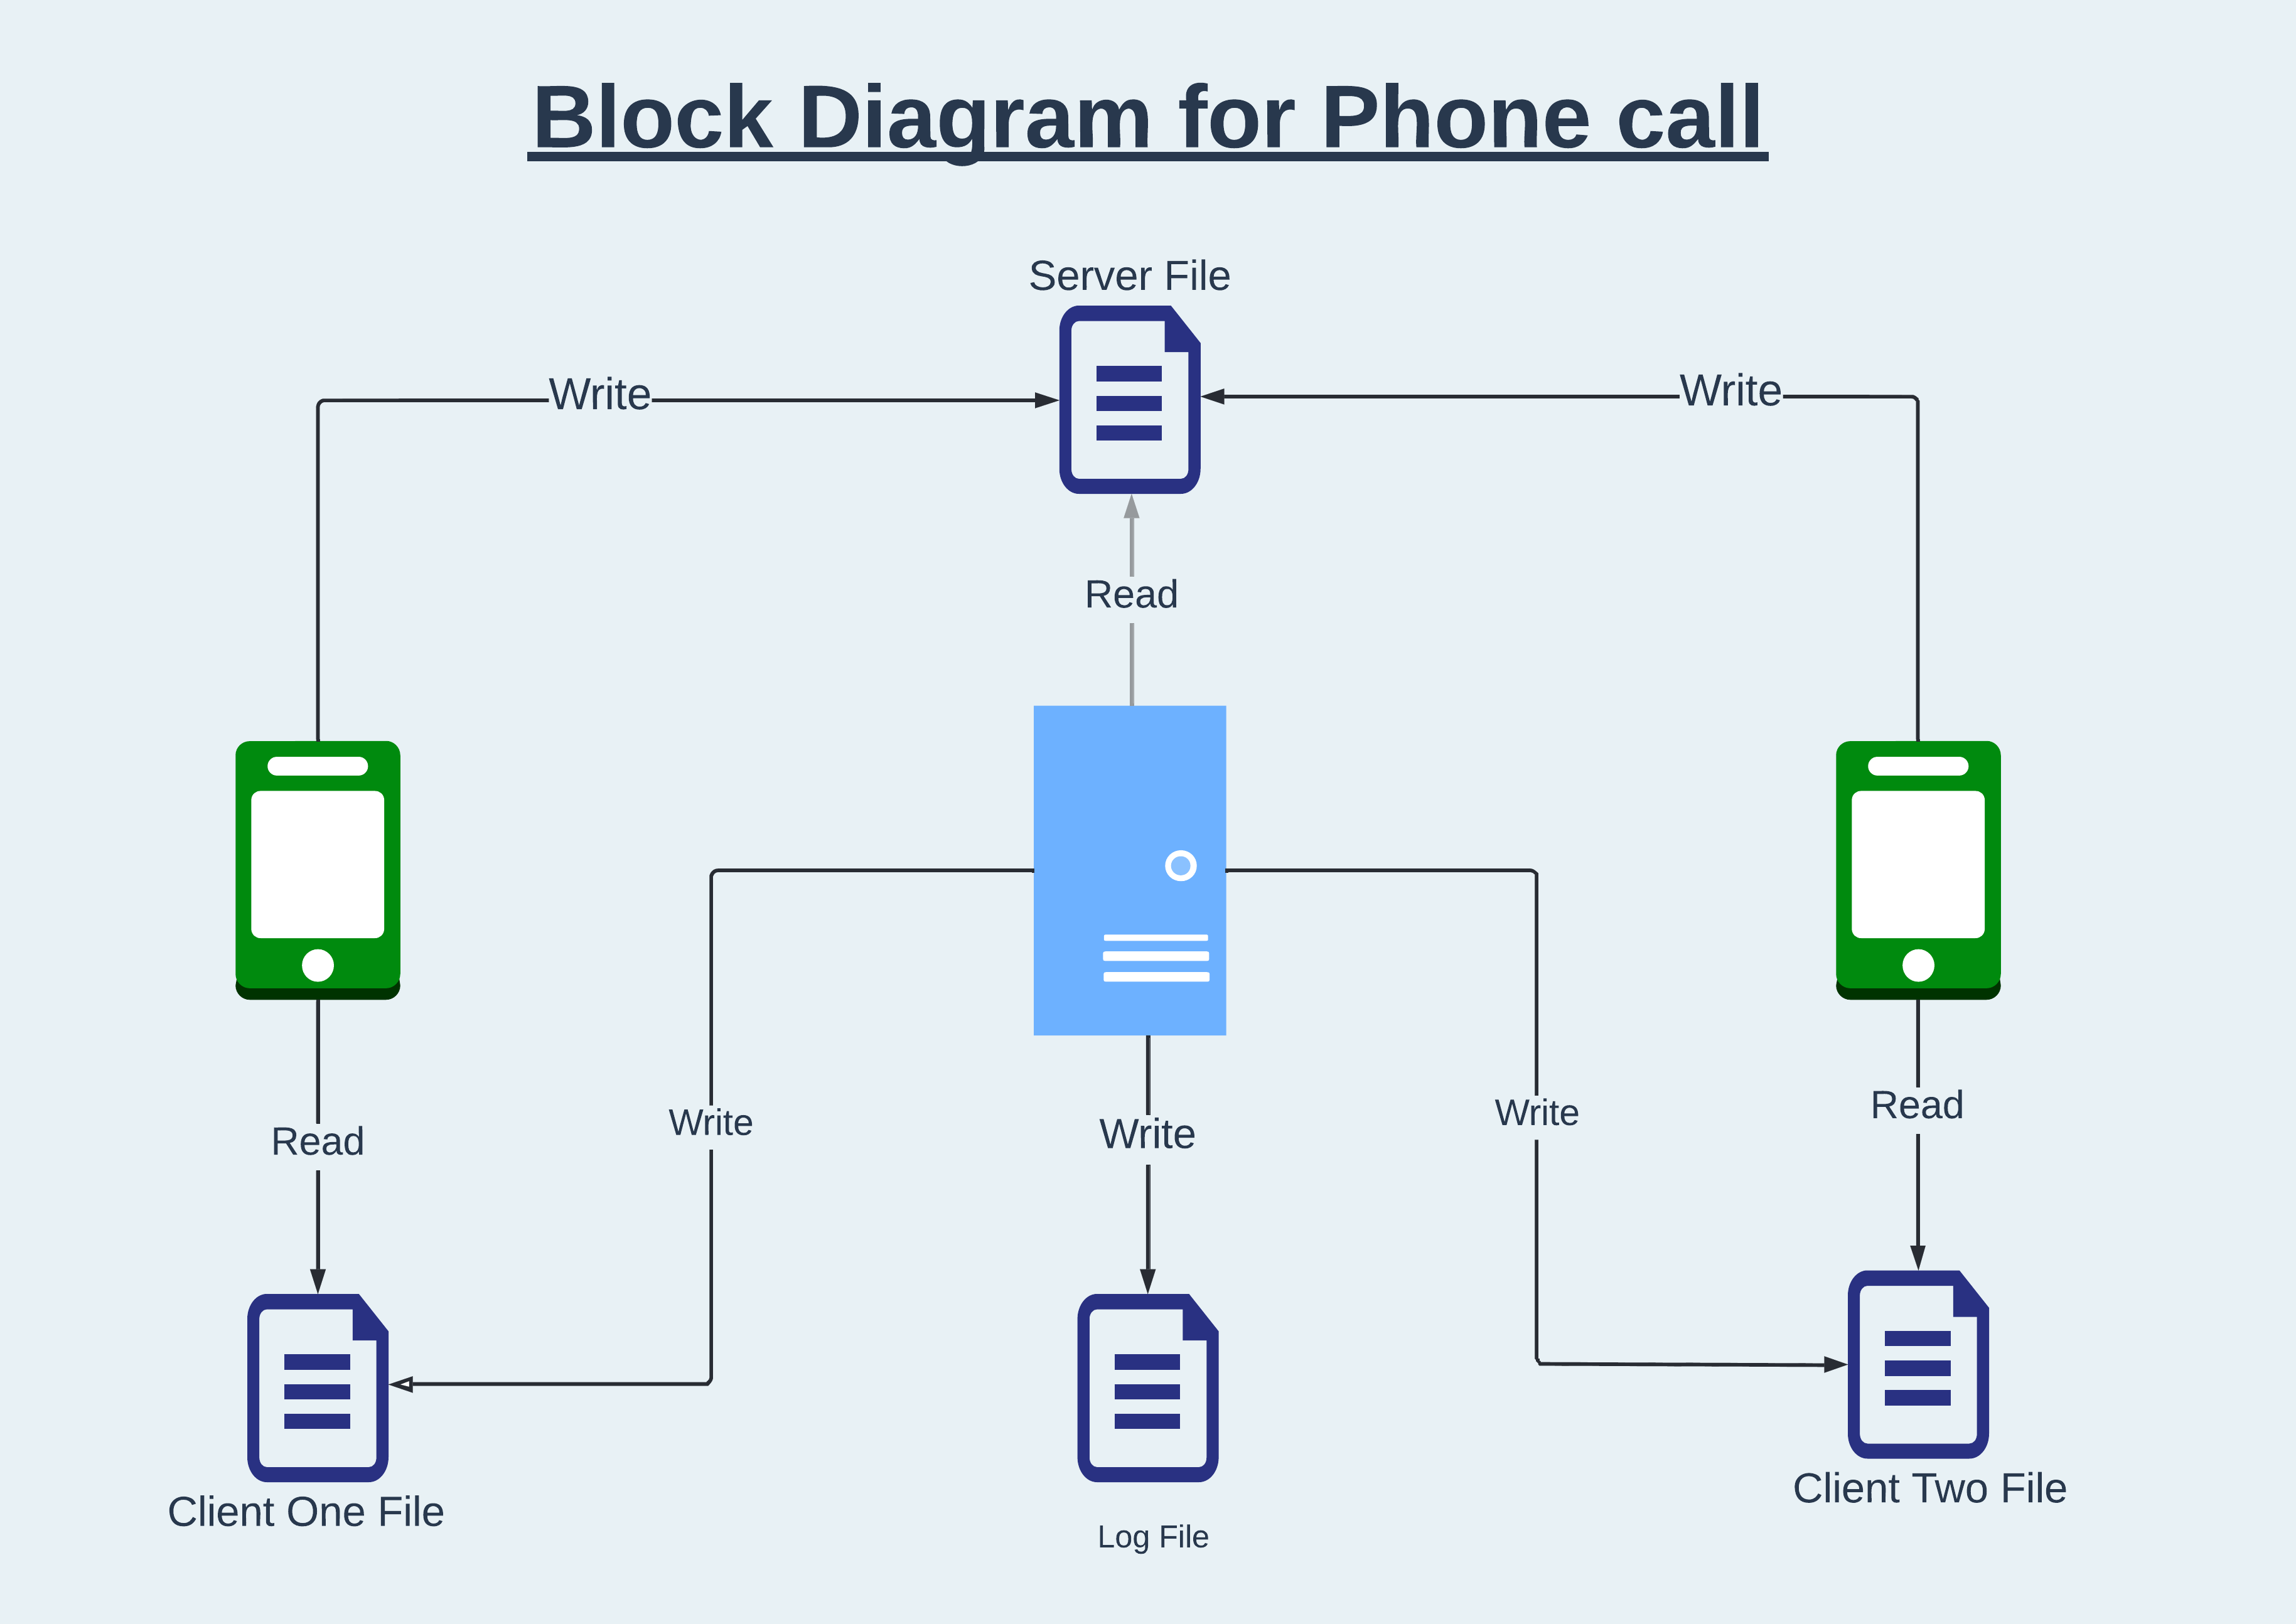
\includegraphics[width=450px, height=300px]{"../../resources/images/project/project-block_diagram.png"}
    }

}

%% Results %% 

\newpage{

    \setlength{\parindent}{0pt}
    \begin{center}
        \textbf{ {\section*{\huge {Results}}}}
    \end{center}

    \LARGE{


    }

}

%% Problem Faced and Solutions %% 

\newpage{

    \setlength{\parindent}{0pt}
    \begin{center}
        \textbf{ {\section*{\huge {Problem Faced and Solutions}}}}
    \end{center}

    \LARGE{
        \justify With every project comes coding, debugging and main fixing bugs. During this project as well, we had to go through  a lot of problems. Using networing in SDL2 was getting hard as there are no much resources for SDL2 unlike SFML.

        \justify Audio processing was begin difficult to execute so instead linux system command is used to record audio in .wav file which is futher processed by server and finally played from called person.

        \justify Dialpad number verifying whether the number is correct or not for call to take place was a little difficult part along with rendering different texture to be displayed in different window.

        \justify This project contains a lot of winodows and texture rendering which was sometime gettting confused and time consuming to debug even simple errors.

        \justify Though facing all this problems, the project was completed with effort.
    }

}

%% Limitation and Future Enhancement %% 

\newpage{

    \setlength{\parindent}{0pt}
    \begin{center}
        \textbf{ {\section*{\huge {Limitation and Future Enhancement}}}}
    \end{center}

    \LARGE{
        \textbf{Limitations: \\}
        - It doesn't fully model the real phone call simulation but has most of it with limited feactures to demostrate everything in good manner. \\
        - Recording audio part was done using linux system commands so this project will only work in linux os. \\
        - As a server, different file concept was just. Eg: server writing the message in clients txt which is processed by continuing loop of client and respective task being done in client window.

        \textbf{Future Enhancement: \\}
        - Use of more advanced library can give this project a better server networking and LAN netowrking which could make the simulation more realistic in small space frame like wireless and bluetooth facility.
        - Sending audio using networking and wireless media would be more better.
        - Making this project to run in mobile as an application would be great and practial matching.
    }

}

%% Conclusion and Recommendations %% 

\newpage{

    \setlength{\parindent}{0pt}
    \begin{center}
        \textbf{ {\section*{\huge {Conclusion and Recommendations}}}}
    \end{center}

    \LARGE{
    }

}

%% References %%

\newpage{

    \setlength{\parindent}{0pt}
    \begin{center}
        \textbf{ {\section*{\huge {References}}}}
    \end{center}
    \LARGE{
    }

}



\end{document}
